\documentclass[1p]{elsarticle_modified}
%\bibliographystyle{elsarticle-num}

%\usepackage[colorlinks]{hyperref}
%\usepackage{abbrmath_seonhwa} %\Abb, \Ascr, \Acal ,\Abf, \Afrak
\usepackage{amsfonts}
\usepackage{amssymb}
\usepackage{amsmath}
\usepackage{amsthm}
\usepackage{scalefnt}
\usepackage{amsbsy}
\usepackage{kotex}
\usepackage{caption}
\usepackage{subfig}
\usepackage{color}
\usepackage{graphicx}
\usepackage{xcolor} %% white, black, red, green, blue, cyan, magenta, yellow
\usepackage{float}
\usepackage{setspace}
\usepackage{hyperref}

\usepackage{tikz}
\usetikzlibrary{arrows}

\usepackage{multirow}
\usepackage{array} % fixed length table
\usepackage{hhline}

%%%%%%%%%%%%%%%%%%%%%
\makeatletter
\renewcommand*\env@matrix[1][\arraystretch]{%
	\edef\arraystretch{#1}%
	\hskip -\arraycolsep
	\let\@ifnextchar\new@ifnextchar
	\array{*\c@MaxMatrixCols c}}
\makeatother %https://tex.stackexchange.com/questions/14071/how-can-i-increase-the-line-spacing-in-a-matrix
%%%%%%%%%%%%%%%

\usepackage[normalem]{ulem}

\newcommand{\msout}[1]{\ifmmode\text{\sout{\ensuremath{#1}}}\else\sout{#1}\fi}
%SOURCE: \msout is \stkout macro in https://tex.stackexchange.com/questions/20609/strikeout-in-math-mode

\newcommand{\cancel}[1]{
	\ifmmode
	{\color{red}\msout{#1}}
	\else
	{\color{red}\sout{#1}}
	\fi
}

\newcommand{\add}[1]{
	{\color{blue}\uwave{#1}}
}

\newcommand{\replace}[2]{
	\ifmmode
	{\color{red}\msout{#1}}{\color{blue}\uwave{#2}}
	\else
	{\color{red}\sout{#1}}{\color{blue}\uwave{#2}}
	\fi
}

\newcommand{\Sol}{\mathcal{S}} %segment
\newcommand{\D}{D} %diagram
\newcommand{\A}{\mathcal{A}} %arc


%%%%%%%%%%%%%%%%%%%%%%%%%%%%%5 test

\def\sl{\operatorname{\textup{SL}}(2,\Cbb)}
\def\psl{\operatorname{\textup{PSL}}(2,\Cbb)}
\def\quan{\mkern 1mu \triangleright \mkern 1mu}

\theoremstyle{definition}
\newtheorem{thm}{Theorem}[section]
\newtheorem{prop}[thm]{Proposition}
\newtheorem{lem}[thm]{Lemma}
\newtheorem{ques}[thm]{Question}
\newtheorem{cor}[thm]{Corollary}
\newtheorem{defn}[thm]{Definition}
\newtheorem{exam}[thm]{Example}
\newtheorem{rmk}[thm]{Remark}
\newtheorem{alg}[thm]{Algorithm}

\newcommand{\I}{\sqrt{-1}}
\begin{document}

%\begin{frontmatter}
%
%\title{Boundary parabolic representations of knots up to 8 crossings}
%
%%% Group authors per affiliation:
%\author{Yunhi Cho} 
%\address{Department of Mathematics, University of Seoul, Seoul, Korea}
%\ead{yhcho@uos.ac.kr}
%
%
%\author{Seonhwa Kim} %\fnref{s_kim}}
%\address{Center for Geometry and Physics, Institute for Basic Science, Pohang, 37673, Korea}
%\ead{ryeona17@ibs.re.kr}
%
%\author{Hyuk Kim}
%\address{Department of Mathematical Sciences, Seoul National University, Seoul 08826, Korea}
%\ead{hyukkim@snu.ac.kr}
%
%\author{Seokbeom Yoon}
%\address{Department of Mathematical Sciences, Seoul National University, Seoul, 08826,  Korea}
%\ead{sbyoon15@snu.ac.kr}
%
%\begin{abstract}
%We find all boundary parabolic representation of knots up to 8 crossings.
%
%\end{abstract}
%\begin{keyword}
%    \MSC[2010] 57M25 
%\end{keyword}
%
%\end{frontmatter}

%\linenumbers
%\tableofcontents
%
\newcommand\colored[1]{\textcolor{white}{\rule[-0.35ex]{0.8em}{1.4ex}}\kern-0.8em\color{red} #1}%
%\newcommand\colored[1]{\textcolor{white}{ #1}\kern-2.17ex	\textcolor{white}{ #1}\kern-1.81ex	\textcolor{white}{ #1}\kern-2.15ex\color{red}#1	}

{\Large $\underline{12n_{0267}~(K12n_{0267})}$}

\setlength{\tabcolsep}{10pt}
\renewcommand{\arraystretch}{1.6}
\vspace{1cm}\begin{tabular}{m{100pt}>{\centering\arraybackslash}m{274pt}}
\multirow{5}{120pt}{
	\centering
	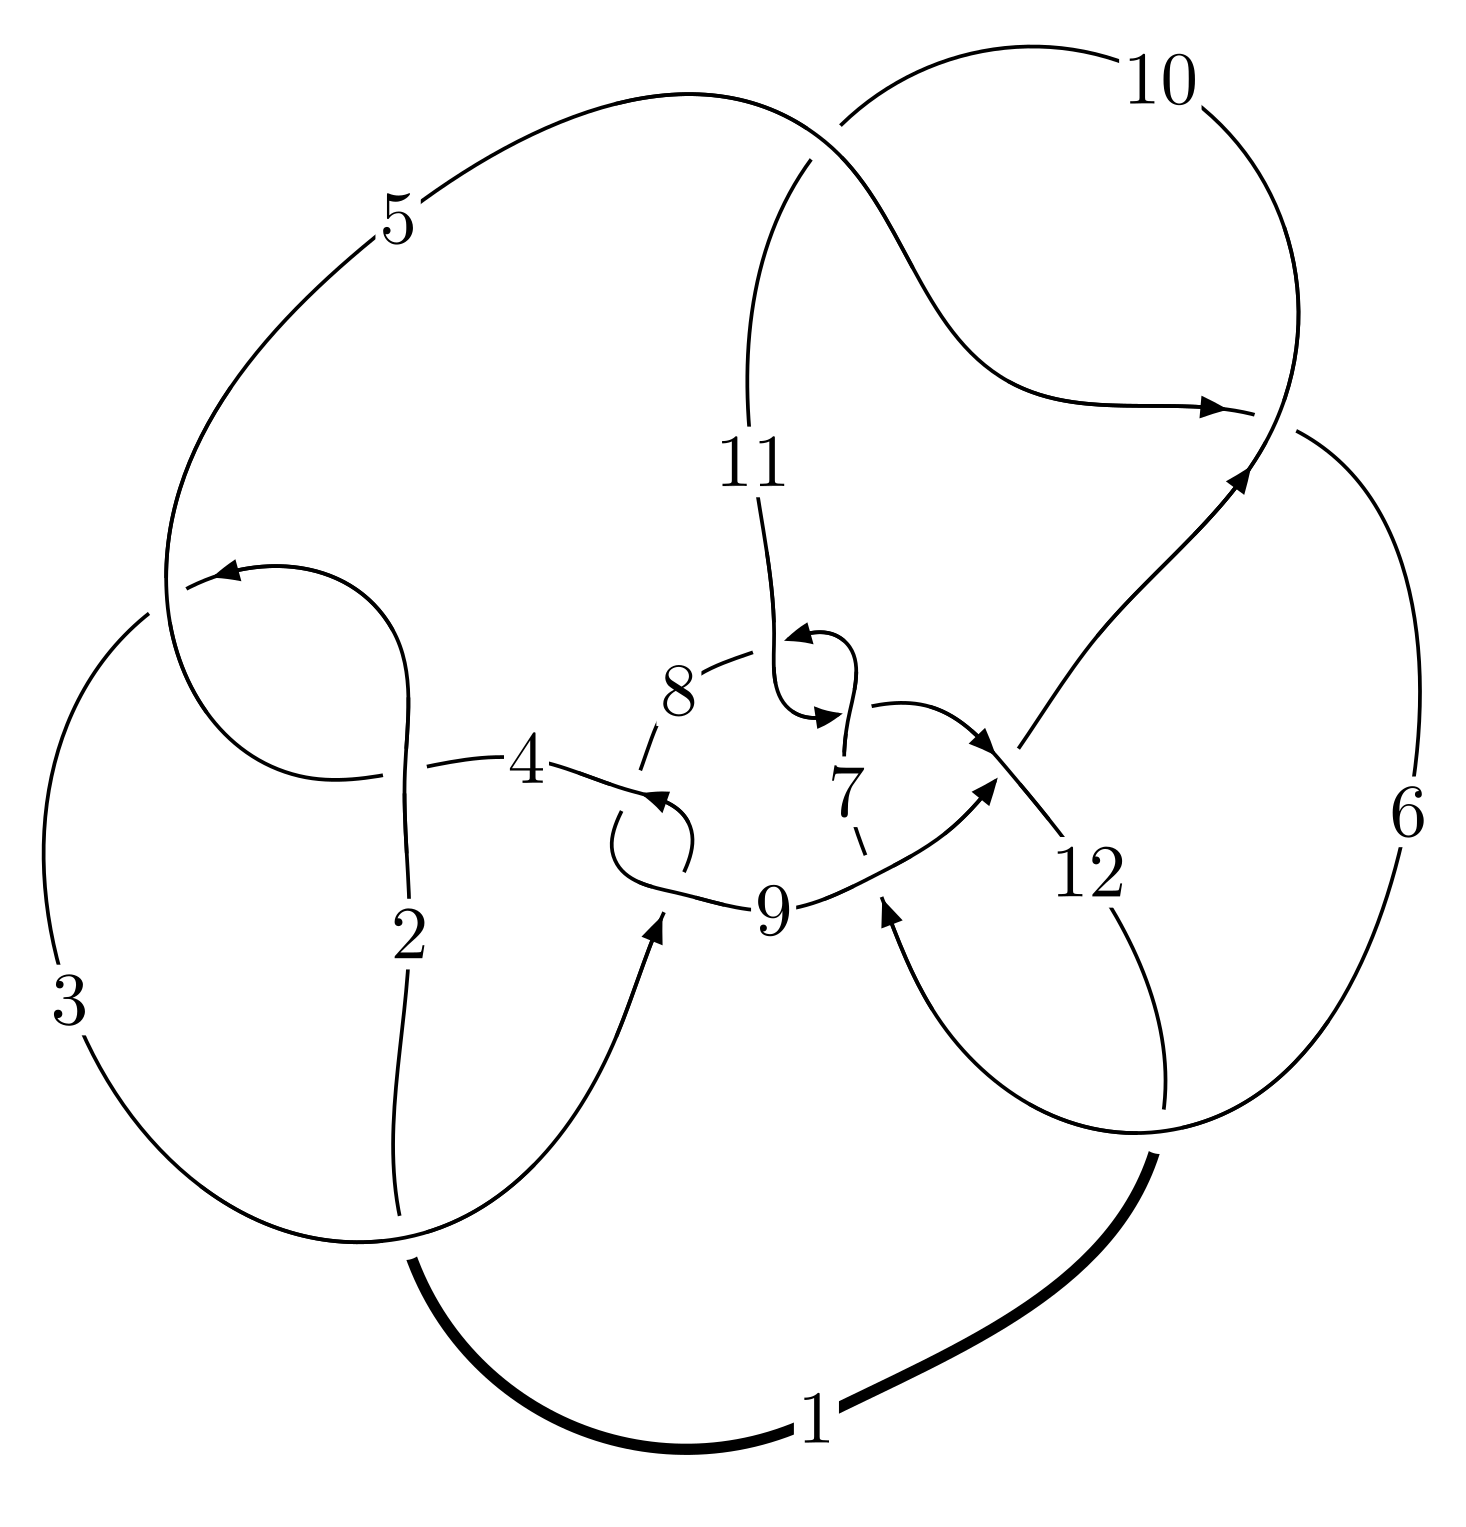
\includegraphics[width=112pt]{../../../GIT/diagram.site/Diagrams/png/2356_12n_0267.png}\\
\ \ \ A knot diagram\footnotemark}&
\allowdisplaybreaks
\textbf{Linearized knot diagam} \\
\cline{2-2}
 &
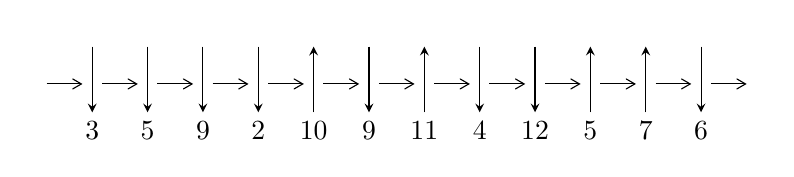
\begin{tikzpicture}[x=20pt, y=17pt]
	% nodes
	\node (C0) at (0, 0) {};
	\node (C1) at (1, 0) {};
	\node (C1U) at (1, +1) {};
	\node (C1D) at (1, -1) {3};

	\node (C2) at (2, 0) {};
	\node (C2U) at (2, +1) {};
	\node (C2D) at (2, -1) {5};

	\node (C3) at (3, 0) {};
	\node (C3U) at (3, +1) {};
	\node (C3D) at (3, -1) {9};

	\node (C4) at (4, 0) {};
	\node (C4U) at (4, +1) {};
	\node (C4D) at (4, -1) {2};

	\node (C5) at (5, 0) {};
	\node (C5U) at (5, +1) {};
	\node (C5D) at (5, -1) {10};

	\node (C6) at (6, 0) {};
	\node (C6U) at (6, +1) {};
	\node (C6D) at (6, -1) {9};

	\node (C7) at (7, 0) {};
	\node (C7U) at (7, +1) {};
	\node (C7D) at (7, -1) {11};

	\node (C8) at (8, 0) {};
	\node (C8U) at (8, +1) {};
	\node (C8D) at (8, -1) {4};

	\node (C9) at (9, 0) {};
	\node (C9U) at (9, +1) {};
	\node (C9D) at (9, -1) {12};

	\node (C10) at (10, 0) {};
	\node (C10U) at (10, +1) {};
	\node (C10D) at (10, -1) {5};

	\node (C11) at (11, 0) {};
	\node (C11U) at (11, +1) {};
	\node (C11D) at (11, -1) {7};

	\node (C12) at (12, 0) {};
	\node (C12U) at (12, +1) {};
	\node (C12D) at (12, -1) {6};
	\node (C13) at (13, 0) {};

	% arrows
	\draw[->,>={angle 60}]
	(C0) edge (C1) (C1) edge (C2) (C2) edge (C3) (C3) edge (C4) (C4) edge (C5) (C5) edge (C6) (C6) edge (C7) (C7) edge (C8) (C8) edge (C9) (C9) edge (C10) (C10) edge (C11) (C11) edge (C12) (C12) edge (C13) ;	\draw[->,>=stealth]
	(C1U) edge (C1D) (C2U) edge (C2D) (C3U) edge (C3D) (C4U) edge (C4D) (C5D) edge (C5U) (C6U) edge (C6D) (C7D) edge (C7U) (C8U) edge (C8D) (C9U) edge (C9D) (C10D) edge (C10U) (C11D) edge (C11U) (C12U) edge (C12D) ;
	\end{tikzpicture} \\
\hhline{~~} \\& 
\textbf{Solving Sequence} \\ \cline{2-2} 
 &
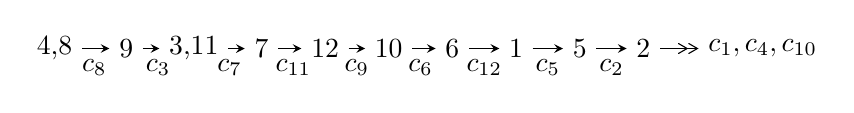
\begin{tikzpicture}[x=23pt, y=7pt]
	% node
	\node (A0) at (-1/8, 0) {4,8};
	\node (A1) at (1, 0) {9};
	\node (A2) at (33/16, 0) {3,11};
	\node (A3) at (25/8, 0) {7};
	\node (A4) at (33/8, 0) {12};
	\node (A5) at (41/8, 0) {10};
	\node (A6) at (49/8, 0) {6};
	\node (A7) at (57/8, 0) {1};
	\node (A8) at (65/8, 0) {5};
	\node (A9) at (73/8, 0) {2};
	\node (C1) at (1/2, -1) {$c_{8}$};
	\node (C2) at (3/2, -1) {$c_{3}$};
	\node (C3) at (21/8, -1) {$c_{7}$};
	\node (C4) at (29/8, -1) {$c_{11}$};
	\node (C5) at (37/8, -1) {$c_{9}$};
	\node (C6) at (45/8, -1) {$c_{6}$};
	\node (C7) at (53/8, -1) {$c_{12}$};
	\node (C8) at (61/8, -1) {$c_{5}$};
	\node (C9) at (69/8, -1) {$c_{2}$};
	\node (A10) at (11, 0) {$c_{1},c_{4},c_{10}$};

	% edge
	\draw[->,>=stealth]	
	(A0) edge (A1) (A1) edge (A2) (A2) edge (A3) (A3) edge (A4) (A4) edge (A5) (A5) edge (A6) (A6) edge (A7) (A7) edge (A8) (A8) edge (A9) ;
	\draw[->>,>={angle 60}]	
	(A9) edge (A10);
\end{tikzpicture} \\ 

\end{tabular} \\

\footnotetext{
The image of knot diagram is generated by the software ``\textbf{Draw programme}" developed by Andrew Bartholomew(\url{http://www.layer8.co.uk/maths/draw/index.htm\#Running-draw}), where we modified some parts for our purpose(\url{https://github.com/CATsTAILs/LinksPainter}).
}\phantom \\ \newline 
\centering \textbf{Ideals for irreducible components\footnotemark of $X_{\text{par}}$} 
 
\begin{align*}
I^u_{1}&=\langle 
1.63228\times10^{53} u^{27}+1.02544\times10^{54} u^{26}+\cdots+3.06469\times10^{56} b+3.90256\times10^{56},\\
\phantom{I^u_{1}}&\phantom{= \langle  }1.81316\times10^{54} u^{27}+1.29787\times10^{55} u^{26}+\cdots+2.45175\times10^{57} a-9.42098\times10^{56},\\
\phantom{I^u_{1}}&\phantom{= \langle  }u^{28}+7 u^{27}+\cdots-256 u-1024\rangle \\
I^u_{2}&=\langle 
-15 a^5 u^4-35 a^4 u^4+\cdots+62 a+18,\;12 a^5 u^4+166 a^4 u^4+\cdots+144010 a+300665,\\
\phantom{I^u_{2}}&\phantom{= \langle  }u^5- u^4+5 u^3- u^2+2 u+2\rangle \\
I^u_{3}&=\langle 
-2796800274 u^{16}+1230170348 u^{15}+\cdots+5782655035 b+1488757467,\\
\phantom{I^u_{3}}&\phantom{= \langle  }-115474 u^{16}+4433863 u^{15}+\cdots+2844395 a-26311393,\;u^{17}+6 u^{15}+\cdots-3 u-1\rangle \\
\\
I^v_{1}&=\langle 
a,\;8 v^3-12 v^2+b+10 v-3,\;8 v^4-12 v^3+12 v^2-5 v+1\rangle \\
I^v_{2}&=\langle 
a,\;b^6- b^5+2 b^4-2 b^3+2 b^2-2 b+1,\;v+1\rangle \\
\end{align*}
\raggedright * 5 irreducible components of $\dim_{\mathbb{C}}=0$, with total 85 representations.\\
\footnotetext{All coefficients of polynomials are rational numbers. But the coefficients are sometimes approximated in decimal forms when there is not enough margin.}
\newpage
\renewcommand{\arraystretch}{1}
\centering \section*{I. $I^u_{1}= \langle 1.63\times10^{53} u^{27}+1.03\times10^{54} u^{26}+\cdots+3.06\times10^{56} b+3.90\times10^{56},\;1.81\times10^{54} u^{27}+1.30\times10^{55} u^{26}+\cdots+2.45\times10^{57} a-9.42\times10^{56},\;u^{28}+7 u^{27}+\cdots-256 u-1024 \rangle$}
\flushleft \textbf{(i) Arc colorings}\\
\begin{tabular}{m{7pt} m{180pt} m{7pt} m{180pt} }
\flushright $a_{4}=$&$\begin{pmatrix}0\\u\end{pmatrix}$ \\
\flushright $a_{8}=$&$\begin{pmatrix}1\\0\end{pmatrix}$ \\
\flushright $a_{9}=$&$\begin{pmatrix}1\\u^2\end{pmatrix}$ \\
\flushright $a_{3}=$&$\begin{pmatrix}u\\u^3+u\end{pmatrix}$ \\
\flushright $a_{11}=$&$\begin{pmatrix}-0.000739535 u^{27}-0.00529364 u^{26}+\cdots+1.32145 u+0.384255\\-0.000532608 u^{27}-0.00334597 u^{26}+\cdots-0.222903 u-1.27339\end{pmatrix}$ \\
\flushright $a_{7}=$&$\begin{pmatrix}-0.0000164451 u^{27}-0.000139457 u^{26}+\cdots+0.107664 u+0.565098\\-0.000174750 u^{27}-0.00136950 u^{26}+\cdots-0.302799 u-0.594774\end{pmatrix}$ \\
\flushright $a_{12}=$&$\begin{pmatrix}-0.000886322 u^{27}-0.00613088 u^{26}+\cdots+1.06551 u-0.306723\\-0.000917462 u^{27}-0.00664824 u^{26}+\cdots+2.05507 u-0.158393\end{pmatrix}$ \\
\flushright $a_{10}=$&$\begin{pmatrix}-0.000128059 u^{27}-0.000962696 u^{26}+\cdots+0.904215 u+1.23308\\0.000823960 u^{27}+0.00616689 u^{26}+\cdots-1.24171 u-0.0314143\end{pmatrix}$ \\
\flushright $a_{6}=$&$\begin{pmatrix}-0.000282712 u^{27}-0.00211501 u^{26}+\cdots-0.172064 u-0.00475082\\-0.000128885 u^{27}-0.000876415 u^{26}+\cdots-0.604047 u-0.709139\end{pmatrix}$ \\
\flushright $a_{1}=$&$\begin{pmatrix}-0.000661565 u^{27}-0.00488332 u^{26}+\cdots+2.13497 u+0.559124\\-0.000843467 u^{27}-0.00643716 u^{26}+\cdots+3.43637 u+0.641978\end{pmatrix}$ \\
\flushright $a_{5}=$&$\begin{pmatrix}0.000363425 u^{27}+0.00276215 u^{26}+\cdots-2.04345 u-0.341280\\0.00102499 u^{27}+0.00764547 u^{26}+\cdots-4.17842 u-0.900404\end{pmatrix}$ \\
\flushright $a_{2}=$&$\begin{pmatrix}-0.000405455 u^{27}-0.00320663 u^{26}+\cdots+2.56297 u+0.782535\\-0.000623273 u^{27}-0.00509696 u^{26}+\cdots+4.09691 u+0.746524\end{pmatrix}$\\&\end{tabular}
\flushleft \textbf{(ii) Obstruction class $= -1$}\\~\\
\flushleft \textbf{(iii) Cusp Shapes $= 0.000805991 u^{27}+0.000903953 u^{26}+\cdots+16.6786 u+9.73356$}\\~\\
\newpage\renewcommand{\arraystretch}{1}
\flushleft \textbf{(iv) u-Polynomials at the component}\newline \\
\begin{tabular}{m{50pt}|m{274pt}}
Crossings & \hspace{64pt}u-Polynomials at each crossing \\
\hline $$\begin{aligned}c_{1}\end{aligned}$$&$\begin{aligned}
&u^{28}+11 u^{27}+\cdots+38144 u+4096
\end{aligned}$\\
\hline $$\begin{aligned}c_{2},c_{4}\end{aligned}$$&$\begin{aligned}
&u^{28}-5 u^{27}+\cdots+368 u-64
\end{aligned}$\\
\hline $$\begin{aligned}c_{3},c_{8}\end{aligned}$$&$\begin{aligned}
&u^{28}-7 u^{27}+\cdots+256 u-1024
\end{aligned}$\\
\hline $$\begin{aligned}c_{5},c_{7},c_{10}\\c_{11}\end{aligned}$$&$\begin{aligned}
&u^{28}- u^{26}+\cdots+6 u+1
\end{aligned}$\\
\hline $$\begin{aligned}c_{6},c_{12}\end{aligned}$$&$\begin{aligned}
&u^{28}- u^{27}+\cdots+5 u+1
\end{aligned}$\\
\hline $$\begin{aligned}c_{9}\end{aligned}$$&$\begin{aligned}
&u^{28}-11 u^{27}+\cdots-464 u+32
\end{aligned}$\\
\hline
\end{tabular}\\~\\
\newpage\renewcommand{\arraystretch}{1}
\flushleft \textbf{(v) Riley Polynomials at the component}\newline \\
\begin{tabular}{m{50pt}|m{274pt}}
Crossings & \hspace{64pt}Riley Polynomials at each crossing \\
\hline $$\begin{aligned}c_{1}\end{aligned}$$&$\begin{aligned}
&y^{28}+17 y^{27}+\cdots-423952384 y+16777216
\end{aligned}$\\
\hline $$\begin{aligned}c_{2},c_{4}\end{aligned}$$&$\begin{aligned}
&y^{28}-11 y^{27}+\cdots-38144 y+4096
\end{aligned}$\\
\hline $$\begin{aligned}c_{3},c_{8}\end{aligned}$$&$\begin{aligned}
&y^{28}+21 y^{27}+\cdots+7012352 y+1048576
\end{aligned}$\\
\hline $$\begin{aligned}c_{5},c_{7},c_{10}\\c_{11}\end{aligned}$$&$\begin{aligned}
&y^{28}-2 y^{27}+\cdots-16 y+1
\end{aligned}$\\
\hline $$\begin{aligned}c_{6},c_{12}\end{aligned}$$&$\begin{aligned}
&y^{28}+15 y^{27}+\cdots+59 y+1
\end{aligned}$\\
\hline $$\begin{aligned}c_{9}\end{aligned}$$&$\begin{aligned}
&y^{28}-9 y^{27}+\cdots-57088 y+1024
\end{aligned}$\\
\hline
\end{tabular}\\~\\
\newpage\flushleft \textbf{(vi) Complex Volumes and Cusp Shapes}
$$\begin{array}{c|c|c}  
\text{Solutions to }I^u_{1}& \I (\text{vol} + \sqrt{-1}CS) & \text{Cusp shape}\\
 \hline 
\begin{aligned}
u &= -0.700519 + 0.599156 I \\
a &= \phantom{-}0.801515 - 1.064090 I \\
b &= \phantom{-}0.037633 - 0.642247 I\end{aligned}
 & -3.55837 - 1.15126 I & -11.39772 - 0.05458 I \\ \hline\begin{aligned}
u &= -0.700519 - 0.599156 I \\
a &= \phantom{-}0.801515 + 1.064090 I \\
b &= \phantom{-}0.037633 + 0.642247 I\end{aligned}
 & -3.55837 + 1.15126 I & -11.39772 + 0.05458 I \\ \hline\begin{aligned}
u &= \phantom{-}0.380572 + 0.813474 I \\
a &= \phantom{-}0.564232 + 0.751884 I \\
b &= -0.166171 + 0.662526 I\end{aligned}
 & -0.05630 - 1.72703 I & -1.78795 + 1.55176 I \\ \hline\begin{aligned}
u &= \phantom{-}0.380572 - 0.813474 I \\
a &= \phantom{-}0.564232 - 0.751884 I \\
b &= -0.166171 - 0.662526 I\end{aligned}
 & -0.05630 + 1.72703 I & -1.78795 - 1.55176 I \\ \hline\begin{aligned}
u &= -0.588263 + 1.018270 I \\
a &= \phantom{-}0.470372 - 0.902968 I \\
b &= -0.094878 - 0.756998 I\end{aligned}
 & -2.26210 + 6.12921 I & -7.94602 + 0.52990 I \\ \hline\begin{aligned}
u &= -0.588263 - 1.018270 I \\
a &= \phantom{-}0.470372 + 0.902968 I \\
b &= -0.094878 + 0.756998 I\end{aligned}
 & -2.26210 - 6.12921 I & -7.94602 - 0.52990 I \\ \hline\begin{aligned}
u &= \phantom{-}1.069010 + 0.807521 I \\
a &= -0.138524 - 0.648901 I \\
b &= \phantom{-}0.903329 - 0.048342 I\end{aligned}
 & -0.304442 - 0.720791 I & -1.85900 + 1.85047 I \\ \hline\begin{aligned}
u &= \phantom{-}1.069010 - 0.807521 I \\
a &= -0.138524 + 0.648901 I \\
b &= \phantom{-}0.903329 + 0.048342 I\end{aligned}
 & -0.304442 + 0.720791 I & -1.85900 - 1.85047 I \\ \hline\begin{aligned}
u &= \phantom{-}0.289195 + 0.590850 I \\
a &= -0.185649 - 0.370483 I \\
b &= \phantom{-}0.454678 - 1.109670 I\end{aligned}
 & -4.11561 - 8.14651 I & -4.6236 + 14.7439 I \\ \hline\begin{aligned}
u &= \phantom{-}0.289195 - 0.590850 I \\
a &= -0.185649 + 0.370483 I \\
b &= \phantom{-}0.454678 + 1.109670 I\end{aligned}
 & -4.11561 + 8.14651 I & -4.6236 - 14.7439 I\\
 \hline 
 \end{array}$$\newpage$$\begin{array}{c|c|c}  
\text{Solutions to }I^u_{1}& \I (\text{vol} + \sqrt{-1}CS) & \text{Cusp shape}\\
 \hline 
\begin{aligned}
u &= -0.008090 + 0.619126 I \\
a &= \phantom{-}0.445860 + 0.546608 I \\
b &= -0.405809 + 0.656851 I\end{aligned}
 & \phantom{-}0.33084 - 1.64029 I & \phantom{-}3.18047 + 4.70949 I \\ \hline\begin{aligned}
u &= -0.008090 - 0.619126 I \\
a &= \phantom{-}0.445860 - 0.546608 I \\
b &= -0.405809 - 0.656851 I\end{aligned}
 & \phantom{-}0.33084 + 1.64029 I & \phantom{-}3.18047 - 4.70949 I \\ \hline\begin{aligned}
u &= -1.31770 + 0.54916 I \\
a &= \phantom{-}0.352145 - 0.329705 I \\
b &= -1.100510 - 0.409135 I\end{aligned}
 & \phantom{-}3.36539 + 1.37186 I & -0.78063 - 1.56765 I \\ \hline\begin{aligned}
u &= -1.31770 - 0.54916 I \\
a &= \phantom{-}0.352145 + 0.329705 I \\
b &= -1.100510 + 0.409135 I\end{aligned}
 & \phantom{-}3.36539 - 1.37186 I & -0.78063 + 1.56765 I \\ \hline\begin{aligned}
u &= \phantom{-}0.535945\phantom{ +0.000000I} \\
a &= \phantom{-}1.11271\phantom{ +0.000000I} \\
b &= \phantom{-}0.260909\phantom{ +0.000000I}\end{aligned}
 & -1.18275\phantom{ +0.000000I} & -7.92670\phantom{ +0.000000I} \\ \hline\begin{aligned}
u &= \phantom{-}0.66539 + 1.38340 I \\
a &= \phantom{-}0.420370 + 0.447189 I \\
b &= -0.979556 - 0.414826 I\end{aligned}
 & -0.93155 + 4.11677 I & -2.65942 - 4.73683 I \\ \hline\begin{aligned}
u &= \phantom{-}0.66539 - 1.38340 I \\
a &= \phantom{-}0.420370 - 0.447189 I \\
b &= -0.979556 + 0.414826 I\end{aligned}
 & -0.93155 - 4.11677 I & -2.65942 + 4.73683 I \\ \hline\begin{aligned}
u &= -1.68431\phantom{ +0.000000I} \\
a &= \phantom{-}0.112961\phantom{ +0.000000I} \\
b &= \phantom{-}0.309973\phantom{ +0.000000I}\end{aligned}
 & -10.2990\phantom{ +0.000000I} & -65.2260\phantom{ +0.000000I} \\ \hline\begin{aligned}
u &= -1.70473 + 0.38435 I \\
a &= -0.204716 + 0.352722 I \\
b &= \phantom{-}1.155650 + 0.736871 I\end{aligned}
 & \phantom{-}2.18156 + 7.22574 I & -3.09669 - 6.28834 I \\ \hline\begin{aligned}
u &= -1.70473 - 0.38435 I \\
a &= -0.204716 - 0.352722 I \\
b &= \phantom{-}1.155650 - 0.736871 I\end{aligned}
 & \phantom{-}2.18156 - 7.22574 I & -3.09669 + 6.28834 I\\
 \hline 
 \end{array}$$\newpage$$\begin{array}{c|c|c}  
\text{Solutions to }I^u_{1}& \I (\text{vol} + \sqrt{-1}CS) & \text{Cusp shape}\\
 \hline 
\begin{aligned}
u &= -0.73389 + 1.71578 I \\
a &= -1.098300 + 0.366340 I \\
b &= \phantom{-}1.02566 + 1.08507 I\end{aligned}
 & \phantom{-}9.85046 + 9.25719 I & -3.57812 - 5.07121 I \\ \hline\begin{aligned}
u &= -0.73389 - 1.71578 I \\
a &= -1.098300 - 0.366340 I \\
b &= \phantom{-}1.02566 - 1.08507 I\end{aligned}
 & \phantom{-}9.85046 - 9.25719 I & -3.57812 + 5.07121 I \\ \hline\begin{aligned}
u &= -0.84442 + 1.78161 I \\
a &= \phantom{-}1.062890 - 0.293393 I \\
b &= -1.07966 - 1.38439 I\end{aligned}
 & \phantom{-}8.3503 + 16.4009 I & -4.99450 - 7.83007 I \\ \hline\begin{aligned}
u &= -0.84442 - 1.78161 I \\
a &= \phantom{-}1.062890 + 0.293393 I \\
b &= -1.07966 + 1.38439 I\end{aligned}
 & \phantom{-}8.3503 - 16.4009 I & -4.99450 + 7.83007 I \\ \hline\begin{aligned}
u &= \phantom{-}0.22185 + 2.03555 I \\
a &= -0.956969 - 0.026772 I \\
b &= \phantom{-}1.27197 - 0.92548 I\end{aligned}
 & \phantom{-}11.43660 - 1.44441 I & -1.83528 + 0. I\phantom{ +0.000000I} \\ \hline\begin{aligned}
u &= \phantom{-}0.22185 - 2.03555 I \\
a &= -0.956969 + 0.026772 I \\
b &= \phantom{-}1.27197 + 0.92548 I\end{aligned}
 & \phantom{-}11.43660 + 1.44441 I & -1.83528 + 0. I\phantom{ +0.000000I} \\ \hline\begin{aligned}
u &= \phantom{-}0.34578 + 2.17004 I \\
a &= \phantom{-}0.853942 + 0.002644 I \\
b &= -1.30777 + 1.19876 I\end{aligned}
 & \phantom{-}10.24040 - 8.22431 I & -4.00000 + 4.11200 I \\ \hline\begin{aligned}
u &= \phantom{-}0.34578 - 2.17004 I \\
a &= \phantom{-}0.853942 - 0.002644 I \\
b &= -1.30777 - 1.19876 I\end{aligned}
 & \phantom{-}10.24040 + 8.22431 I & -4.00000 - 4.11200 I\\
 \hline 
 \end{array}$$\newpage\newpage\renewcommand{\arraystretch}{1}
\centering \section*{II. $I^u_{2}= \langle -15 a^5 u^4-35 a^4 u^4+\cdots+62 a+18,\;12 a^5 u^4+166 a^4 u^4+\cdots+144010 a+300665,\;u^5- u^4+5 u^3- u^2+2 u+2 \rangle$}
\flushleft \textbf{(i) Arc colorings}\\
\begin{tabular}{m{7pt} m{180pt} m{7pt} m{180pt} }
\flushright $a_{4}=$&$\begin{pmatrix}0\\u\end{pmatrix}$ \\
\flushright $a_{8}=$&$\begin{pmatrix}1\\0\end{pmatrix}$ \\
\flushright $a_{9}=$&$\begin{pmatrix}1\\u^2\end{pmatrix}$ \\
\flushright $a_{3}=$&$\begin{pmatrix}u\\u^3+u\end{pmatrix}$ \\
\flushright $a_{11}=$&$\begin{pmatrix}a\\0.535714 a^{5} u^{4}+1.25000 a^{4} u^{4}+\cdots-2.21429 a-0.642857\end{pmatrix}$ \\
\flushright $a_{7}=$&$\begin{pmatrix}0.607143 a^{5} u^{4}+0.428571 a^{4} u^{4}+\cdots+0.642857 a+2.71429\\-4.67857 a^{5} u^{4}-3.57143 a^{4} u^{4}+\cdots+0.928571 a+3.14286\end{pmatrix}$ \\
\flushright $a_{12}=$&$\begin{pmatrix}-3.71429 a^{5} u^{4}-1.03571 a^{4} u^{4}+\cdots-0.928571 a-2.57143\\16.5714 a^{5} u^{4}+9.71429 a^{4} u^{4}+\cdots-7.71429 a-5.42857\end{pmatrix}$ \\
\flushright $a_{10}=$&$\begin{pmatrix}-1.21429 a^{5} u^{4}-0.607143 a^{4} u^{4}+\cdots+2.78571 a+1.42857\\7.07143 a^{5} u^{4}+3.64286 a^{4} u^{4}+\cdots-3.42857 a-2.71429\end{pmatrix}$ \\
\flushright $a_{6}=$&$\begin{pmatrix}0.607143 a^{5} u^{4}+0.428571 a^{4} u^{4}+\cdots+0.642857 a+1.71429\\-4.67857 a^{5} u^{4}-3.57143 a^{4} u^{4}+\cdots+0.928571 a+2.14286\end{pmatrix}$ \\
\flushright $a_{1}=$&$\begin{pmatrix}\frac{1}{4} u^4-\frac{1}{4} u^2+\frac{3}{2} u-\frac{1}{2}\\- u^4+\frac{1}{2} u^3-\frac{1}{2} u^2\end{pmatrix}$ \\
\flushright $a_{5}=$&$\begin{pmatrix}-\frac{1}{2} u^2+\frac{1}{2} u-1\\-\frac{1}{4} u^4-\frac{1}{4} u^2- u-\frac{1}{2}\end{pmatrix}$ \\
\flushright $a_{2}=$&$\begin{pmatrix}-\frac{1}{4} u^4+\frac{1}{2} u^3+\cdots+\frac{3}{2} u-\frac{1}{2}\\\frac{1}{2} u^3-\frac{1}{2} u^2+u\end{pmatrix}$\\&\end{tabular}
\flushleft \textbf{(ii) Obstruction class $= -1$}\\~\\
\flushleft \textbf{(iii) Cusp Shapes $= \frac{17}{7} a^4 u^4+\frac{5}{7} u^4 a^3+\cdots+\frac{22}{7} a-\frac{92}{7}$}\\~\\
\newpage\renewcommand{\arraystretch}{1}
\flushleft \textbf{(iv) u-Polynomials at the component}\newline \\
\begin{tabular}{m{50pt}|m{274pt}}
Crossings & \hspace{64pt}u-Polynomials at each crossing \\
\hline $$\begin{aligned}c_{1}\end{aligned}$$&$\begin{aligned}
&(u^5+6 u^3+u^2- u+1)^6
\end{aligned}$\\
\hline $$\begin{aligned}c_{2},c_{4}\end{aligned}$$&$\begin{aligned}
&(u^5-2 u^4+2 u^3+u^2- u+1)^6
\end{aligned}$\\
\hline $$\begin{aligned}c_{3},c_{8}\end{aligned}$$&$\begin{aligned}
&(u^5+u^4+5 u^3+u^2+2 u-2)^6
\end{aligned}$\\
\hline $$\begin{aligned}c_{5},c_{7},c_{10}\\c_{11}\end{aligned}$$&$\begin{aligned}
&u^{30}-2 u^{29}+\cdots-20 u+137
\end{aligned}$\\
\hline $$\begin{aligned}c_{6},c_{12}\end{aligned}$$&$\begin{aligned}
&u^{30}-6 u^{29}+\cdots+392 u+191
\end{aligned}$\\
\hline $$\begin{aligned}c_{9}\end{aligned}$$&$\begin{aligned}
&(u^3+u^2-1)^{10}
\end{aligned}$\\
\hline
\end{tabular}\\~\\
\newpage\renewcommand{\arraystretch}{1}
\flushleft \textbf{(v) Riley Polynomials at the component}\newline \\
\begin{tabular}{m{50pt}|m{274pt}}
Crossings & \hspace{64pt}Riley Polynomials at each crossing \\
\hline $$\begin{aligned}c_{1}\end{aligned}$$&$\begin{aligned}
&(y^5+12 y^4+34 y^3-13 y^2- y-1)^6
\end{aligned}$\\
\hline $$\begin{aligned}c_{2},c_{4}\end{aligned}$$&$\begin{aligned}
&(y^5+6 y^3- y^2- y-1)^6
\end{aligned}$\\
\hline $$\begin{aligned}c_{3},c_{8}\end{aligned}$$&$\begin{aligned}
&(y^5+9 y^4+27 y^3+23 y^2+8 y-4)^6
\end{aligned}$\\
\hline $$\begin{aligned}c_{5},c_{7},c_{10}\\c_{11}\end{aligned}$$&$\begin{aligned}
&y^{30}+6 y^{29}+\cdots+131668 y+18769
\end{aligned}$\\
\hline $$\begin{aligned}c_{6},c_{12}\end{aligned}$$&$\begin{aligned}
&y^{30}-2 y^{29}+\cdots-47468 y+36481
\end{aligned}$\\
\hline $$\begin{aligned}c_{9}\end{aligned}$$&$\begin{aligned}
&(y^3- y^2+2 y-1)^{10}
\end{aligned}$\\
\hline
\end{tabular}\\~\\
\newpage\flushleft \textbf{(vi) Complex Volumes and Cusp Shapes}
$$\begin{array}{c|c|c}  
\text{Solutions to }I^u_{2}& \I (\text{vol} + \sqrt{-1}CS) & \text{Cusp shape}\\
 \hline 
\begin{aligned}
u &= \phantom{-}0.375669 + 0.888717 I \\
a &= \phantom{-}0.674585 + 0.800660 I \\
b &= -0.250372 + 0.453019 I\end{aligned}
 & -0.05929 - 1.71921 I & -2.12477 + 0.93832 I \\ \hline\begin{aligned}
u &= \phantom{-}0.375669 + 0.888717 I \\
a &= \phantom{-}0.150570 - 0.874514 I \\
b &= -0.372835 - 1.197460 I\end{aligned}
 & -0.05929 + 3.93704 I & -2.12477 - 5.02057 I \\ \hline\begin{aligned}
u &= \phantom{-}0.375669 + 0.888717 I \\
a &= \phantom{-}0.865106 + 0.190043 I \\
b &= -0.079065 - 1.171220 I\end{aligned}
 & -4.19688 + 1.10891 I & -8.65403 - 2.04112 I \\ \hline\begin{aligned}
u &= \phantom{-}0.375669 + 0.888717 I \\
a &= \phantom{-}0.500602 + 0.675276 I \\
b &= -0.122646 + 0.883622 I\end{aligned}
 & -0.05929 - 1.71921 I & -2.12477 + 0.93832 I \\ \hline\begin{aligned}
u &= \phantom{-}0.375669 + 0.888717 I \\
a &= -0.790896 - 0.900150 I \\
b &= \phantom{-}1.154460 + 0.050802 I\end{aligned}
 & -0.05929 + 3.93704 I & -2.12477 - 5.02057 I \\ \hline\begin{aligned}
u &= \phantom{-}0.375669 + 0.888717 I \\
a &= -0.156566 - 0.585774 I \\
b &= \phantom{-}0.62035 + 1.42290 I\end{aligned}
 & -4.19688 + 1.10891 I & -8.65403 - 2.04112 I \\ \hline\begin{aligned}
u &= \phantom{-}0.375669 - 0.888717 I \\
a &= \phantom{-}0.674585 - 0.800660 I \\
b &= -0.250372 - 0.453019 I\end{aligned}
 & -0.05929 + 1.71921 I & -2.12477 - 0.93832 I \\ \hline\begin{aligned}
u &= \phantom{-}0.375669 - 0.888717 I \\
a &= \phantom{-}0.150570 + 0.874514 I \\
b &= -0.372835 + 1.197460 I\end{aligned}
 & -0.05929 - 3.93704 I & -2.12477 + 5.02057 I \\ \hline\begin{aligned}
u &= \phantom{-}0.375669 - 0.888717 I \\
a &= \phantom{-}0.865106 - 0.190043 I \\
b &= -0.079065 + 1.171220 I\end{aligned}
 & -4.19688 - 1.10891 I & -8.65403 + 2.04112 I \\ \hline\begin{aligned}
u &= \phantom{-}0.375669 - 0.888717 I \\
a &= \phantom{-}0.500602 - 0.675276 I \\
b &= -0.122646 - 0.883622 I\end{aligned}
 & -0.05929 + 1.71921 I & -2.12477 - 0.93832 I\\
 \hline 
 \end{array}$$\newpage$$\begin{array}{c|c|c}  
\text{Solutions to }I^u_{2}& \I (\text{vol} + \sqrt{-1}CS) & \text{Cusp shape}\\
 \hline 
\begin{aligned}
u &= \phantom{-}0.375669 - 0.888717 I \\
a &= -0.790896 + 0.900150 I \\
b &= \phantom{-}1.154460 - 0.050802 I\end{aligned}
 & -0.05929 - 3.93704 I & -2.12477 + 5.02057 I \\ \hline\begin{aligned}
u &= \phantom{-}0.375669 - 0.888717 I \\
a &= -0.156566 + 0.585774 I \\
b &= \phantom{-}0.62035 - 1.42290 I\end{aligned}
 & -4.19688 - 1.10891 I & -8.65403 + 2.04112 I \\ \hline\begin{aligned}
u &= -0.504107\phantom{ +0.000000I} \\
a &= -2.97283 + 2.25685 I \\
b &= -0.436616 - 0.497956 I\end{aligned}
 & -3.11432 + 2.82812 I & -13.43328 - 2.97945 I \\ \hline\begin{aligned}
u &= -0.504107\phantom{ +0.000000I} \\
a &= -2.97283 - 2.25685 I \\
b &= -0.436616 + 0.497956 I\end{aligned}
 & -3.11432 - 2.82812 I & -13.43328 + 2.97945 I \\ \hline\begin{aligned}
u &= -0.504107\phantom{ +0.000000I} \\
a &= -2.46586 + 7.51356 I \\
b &= -0.07832 + 1.49767 I\end{aligned}
 & -7.25191\phantom{ +0.000000I} & -19.9625 + 0. I\phantom{ +0.000000I} \\ \hline\begin{aligned}
u &= -0.504107\phantom{ +0.000000I} \\
a &= -2.46586 - 7.51356 I \\
b &= -0.07832 - 1.49767 I\end{aligned}
 & -7.25191\phantom{ +0.000000I} & -19.9625 + 0. I\phantom{ +0.000000I} \\ \hline\begin{aligned}
u &= -0.504107\phantom{ +0.000000I} \\
a &= \phantom{-}1.11141 + 9.05588 I \\
b &= \phantom{-}0.377491 + 0.857286 I\end{aligned}
 & -3.11432 + 2.82812 I & -13.43328 - 2.97945 I \\ \hline\begin{aligned}
u &= -0.504107\phantom{ +0.000000I} \\
a &= \phantom{-}1.11141 - 9.05588 I \\
b &= \phantom{-}0.377491 - 0.857286 I\end{aligned}
 & -3.11432 - 2.82812 I & -13.43328 + 2.97945 I \\ \hline\begin{aligned}
u &= \phantom{-}0.37638 + 2.02979 I \\
a &= -0.941568 - 0.072890 I \\
b &= \phantom{-}0.99031 - 1.34752 I\end{aligned}
 & \phantom{-}9.99924 - 6.95303 I & -3.38420 + 5.13388 I \\ \hline\begin{aligned}
u &= \phantom{-}0.37638 + 2.02979 I \\
a &= \phantom{-}0.895319 + 0.135542 I \\
b &= -1.30155 + 1.31060 I\end{aligned}
 & \phantom{-}9.99924 - 1.29678 I & -3.38420 - 0.82502 I\\
 \hline 
 \end{array}$$\newpage$$\begin{array}{c|c|c}  
\text{Solutions to }I^u_{2}& \I (\text{vol} + \sqrt{-1}CS) & \text{Cusp shape}\\
 \hline 
\begin{aligned}
u &= \phantom{-}0.37638 + 2.02979 I \\
a &= \phantom{-}0.798012 + 0.078062 I \\
b &= -1.64960 + 0.34874 I\end{aligned}
 & \phantom{-}5.86166 - 4.12490 I & -9.91347 + 2.15443 I \\ \hline\begin{aligned}
u &= \phantom{-}0.37638 + 2.02979 I \\
a &= \phantom{-}0.768176 + 0.214026 I \\
b &= -1.60645 - 0.98436 I\end{aligned}
 & \phantom{-}9.99924 - 6.95303 I & -3.38420 + 5.13388 I \\ \hline\begin{aligned}
u &= \phantom{-}0.37638 + 2.02979 I \\
a &= -0.750216 + 0.005392 I \\
b &= \phantom{-}0.616800 - 0.250072 I\end{aligned}
 & \phantom{-}5.86166 - 4.12490 I & -9.91347 + 2.15443 I \\ \hline\begin{aligned}
u &= \phantom{-}0.37638 + 2.02979 I \\
a &= -0.685847 - 0.213681 I \\
b &= \phantom{-}1.13805 + 1.09576 I\end{aligned}
 & \phantom{-}9.99924 - 1.29678 I & -3.38420 - 0.82502 I \\ \hline\begin{aligned}
u &= \phantom{-}0.37638 - 2.02979 I \\
a &= -0.941568 + 0.072890 I \\
b &= \phantom{-}0.99031 + 1.34752 I\end{aligned}
 & \phantom{-}9.99924 + 6.95303 I & -3.38420 - 5.13388 I \\ \hline\begin{aligned}
u &= \phantom{-}0.37638 - 2.02979 I \\
a &= \phantom{-}0.895319 - 0.135542 I \\
b &= -1.30155 - 1.31060 I\end{aligned}
 & \phantom{-}9.99924 + 1.29678 I & -3.38420 + 0.82502 I \\ \hline\begin{aligned}
u &= \phantom{-}0.37638 - 2.02979 I \\
a &= \phantom{-}0.798012 - 0.078062 I \\
b &= -1.64960 - 0.34874 I\end{aligned}
 & \phantom{-}5.86166 + 4.12490 I & -9.91347 - 2.15443 I \\ \hline\begin{aligned}
u &= \phantom{-}0.37638 - 2.02979 I \\
a &= \phantom{-}0.768176 - 0.214026 I \\
b &= -1.60645 + 0.98436 I\end{aligned}
 & \phantom{-}9.99924 + 6.95303 I & -3.38420 - 5.13388 I \\ \hline\begin{aligned}
u &= \phantom{-}0.37638 - 2.02979 I \\
a &= -0.750216 - 0.005392 I \\
b &= \phantom{-}0.616800 + 0.250072 I\end{aligned}
 & \phantom{-}5.86166 + 4.12490 I & -9.91347 - 2.15443 I \\ \hline\begin{aligned}
u &= \phantom{-}0.37638 - 2.02979 I \\
a &= -0.685847 + 0.213681 I \\
b &= \phantom{-}1.13805 - 1.09576 I\end{aligned}
 & \phantom{-}9.99924 + 1.29678 I & -3.38420 + 0.82502 I\\
 \hline 
 \end{array}$$\newpage\newpage\renewcommand{\arraystretch}{1}
\centering \section*{III. $I^u_{3}= \langle -2.80\times10^{9} u^{16}+1.23\times10^{9} u^{15}+\cdots+5.78\times10^{9} b+1.49\times10^{9},\;-1.15\times10^{5} u^{16}+4.43\times10^{6} u^{15}+\cdots+2.84\times10^{6} a-2.63\times10^{7},\;u^{17}+6 u^{15}+\cdots-3 u-1 \rangle$}
\flushleft \textbf{(i) Arc colorings}\\
\begin{tabular}{m{7pt} m{180pt} m{7pt} m{180pt} }
\flushright $a_{4}=$&$\begin{pmatrix}0\\u\end{pmatrix}$ \\
\flushright $a_{8}=$&$\begin{pmatrix}1\\0\end{pmatrix}$ \\
\flushright $a_{9}=$&$\begin{pmatrix}1\\u^2\end{pmatrix}$ \\
\flushright $a_{3}=$&$\begin{pmatrix}u\\u^3+u\end{pmatrix}$ \\
\flushright $a_{11}=$&$\begin{pmatrix}0.0405970 u^{16}-1.55881 u^{15}+\cdots-7.16863 u+9.25026\\0.483653 u^{16}-0.212735 u^{15}+\cdots-1.67509 u-0.257452\end{pmatrix}$ \\
\flushright $a_{7}=$&$\begin{pmatrix}3.74840 u^{16}-2.16144 u^{15}+\cdots-23.4255 u-3.72929\\0.0829079 u^{16}-0.0995122 u^{15}+\cdots-1.83555 u-0.881897\end{pmatrix}$ \\
\flushright $a_{12}=$&$\begin{pmatrix}3.61930 u^{16}-2.25286 u^{15}+\cdots-19.3756 u+0.277471\\0.355787 u^{16}-0.159534 u^{15}+\cdots-2.01409 u-0.833403\end{pmatrix}$ \\
\flushright $a_{10}=$&$\begin{pmatrix}0.164018 u^{16}-1.84216 u^{15}+\cdots-8.28234 u+10.6964\\0.483653 u^{16}-0.212735 u^{15}+\cdots-1.67509 u-0.257452\end{pmatrix}$ \\
\flushright $a_{6}=$&$\begin{pmatrix}3.51603 u^{16}-2.28526 u^{15}+\cdots-22.5251 u-2.44974\\0.290525 u^{16}-0.147505 u^{15}+\cdots-2.43936 u-1.00571\end{pmatrix}$ \\
\flushright $a_{1}=$&$\begin{pmatrix}1.23077 u^{16}-0.226208 u^{15}+\cdots-4.14992 u-2.86754\\0.0648607 u^{16}+0.00369480 u^{15}+\cdots+0.102878 u-0.137290\end{pmatrix}$ \\
\flushright $a_{5}=$&$\begin{pmatrix}-1.08969 u^{16}+0.114263 u^{15}+\cdots+3.70066 u+2.95645\\0.141079 u^{16}-0.111945 u^{15}+\cdots-0.449264 u+0.0889186\end{pmatrix}$ \\
\flushright $a_{2}=$&$\begin{pmatrix}1.18986 u^{16}-0.118103 u^{15}+\cdots-3.40302 u-2.98180\\0.0172629 u^{16}+0.0956716 u^{15}+\cdots+1.13318 u-0.143448\end{pmatrix}$\\&\end{tabular}
\flushleft \textbf{(ii) Obstruction class $= 1$}\\~\\
\flushleft \textbf{(iii) Cusp Shapes $= \frac{44404088866}{5782655035} u^{16}-\frac{1457732737}{5782655035} u^{15}+\cdots-\frac{34652808542}{1156531007} u-\frac{182738550788}{5782655035}$}\\~\\
\newpage\renewcommand{\arraystretch}{1}
\flushleft \textbf{(iv) u-Polynomials at the component}\newline \\
\begin{tabular}{m{50pt}|m{274pt}}
Crossings & \hspace{64pt}u-Polynomials at each crossing \\
\hline $$\begin{aligned}c_{1}\end{aligned}$$&$\begin{aligned}
&u^{17}-8 u^{16}+\cdots+3 u-1
\end{aligned}$\\
\hline $$\begin{aligned}c_{2}\end{aligned}$$&$\begin{aligned}
&u^{17}+6 u^{16}+\cdots+u+1
\end{aligned}$\\
\hline $$\begin{aligned}c_{3}\end{aligned}$$&$\begin{aligned}
&u^{17}+6 u^{15}+\cdots-3 u+1
\end{aligned}$\\
\hline $$\begin{aligned}c_{4}\end{aligned}$$&$\begin{aligned}
&u^{17}-6 u^{16}+\cdots+u-1
\end{aligned}$\\
\hline $$\begin{aligned}c_{5},c_{11}\end{aligned}$$&$\begin{aligned}
&u^{17}+6 u^{15}+\cdots+3 u-1
\end{aligned}$\\
\hline $$\begin{aligned}c_{6},c_{12}\end{aligned}$$&$\begin{aligned}
&u^{17}-3 u^{16}+\cdots+6 u-1
\end{aligned}$\\
\hline $$\begin{aligned}c_{7},c_{10}\end{aligned}$$&$\begin{aligned}
&u^{17}+6 u^{15}+\cdots+3 u+1
\end{aligned}$\\
\hline $$\begin{aligned}c_{8}\end{aligned}$$&$\begin{aligned}
&u^{17}+6 u^{15}+\cdots-3 u-1
\end{aligned}$\\
\hline $$\begin{aligned}c_{9}\end{aligned}$$&$\begin{aligned}
&u^{17}-5 u^{16}+\cdots+5 u-1
\end{aligned}$\\
\hline
\end{tabular}\\~\\
\newpage\renewcommand{\arraystretch}{1}
\flushleft \textbf{(v) Riley Polynomials at the component}\newline \\
\begin{tabular}{m{50pt}|m{274pt}}
Crossings & \hspace{64pt}Riley Polynomials at each crossing \\
\hline $$\begin{aligned}c_{1}\end{aligned}$$&$\begin{aligned}
&y^{17}+8 y^{16}+\cdots-25 y-1
\end{aligned}$\\
\hline $$\begin{aligned}c_{2},c_{4}\end{aligned}$$&$\begin{aligned}
&y^{17}-8 y^{16}+\cdots+3 y-1
\end{aligned}$\\
\hline $$\begin{aligned}c_{3},c_{8}\end{aligned}$$&$\begin{aligned}
&y^{17}+12 y^{16}+\cdots+3 y-1
\end{aligned}$\\
\hline $$\begin{aligned}c_{5},c_{7},c_{10}\\c_{11}\end{aligned}$$&$\begin{aligned}
&y^{17}+12 y^{16}+\cdots-3 y-1
\end{aligned}$\\
\hline $$\begin{aligned}c_{6},c_{12}\end{aligned}$$&$\begin{aligned}
&y^{17}-19 y^{16}+\cdots-2 y-1
\end{aligned}$\\
\hline $$\begin{aligned}c_{9}\end{aligned}$$&$\begin{aligned}
&y^{17}-7 y^{16}+\cdots+17 y-1
\end{aligned}$\\
\hline
\end{tabular}\\~\\
\newpage\flushleft \textbf{(vi) Complex Volumes and Cusp Shapes}
$$\begin{array}{c|c|c}  
\text{Solutions to }I^u_{3}& \I (\text{vol} + \sqrt{-1}CS) & \text{Cusp shape}\\
 \hline 
\begin{aligned}
u &= \phantom{-}0.123817 + 0.916477 I \\
a &= \phantom{-}0.72791 + 1.22000 I \\
b &= -0.302924 + 0.816439 I\end{aligned}
 & -0.67196 - 2.40485 I & -7.80780 + 6.32008 I \\ \hline\begin{aligned}
u &= \phantom{-}0.123817 - 0.916477 I \\
a &= \phantom{-}0.72791 - 1.22000 I \\
b &= -0.302924 - 0.816439 I\end{aligned}
 & -0.67196 + 2.40485 I & -7.80780 - 6.32008 I \\ \hline\begin{aligned}
u &= -0.519605 + 0.973810 I \\
a &= \phantom{-}0.205092 - 1.101040 I \\
b &= -0.199212 - 0.760976 I\end{aligned}
 & -2.24497 + 6.61108 I & -7.2534 - 15.3751 I \\ \hline\begin{aligned}
u &= -0.519605 - 0.973810 I \\
a &= \phantom{-}0.205092 + 1.101040 I \\
b &= -0.199212 + 0.760976 I\end{aligned}
 & -2.24497 - 6.61108 I & -7.2534 + 15.3751 I \\ \hline\begin{aligned}
u &= -0.718697 + 0.273065 I \\
a &= \phantom{-}0.143920 - 1.236700 I \\
b &= -0.503625 + 0.659985 I\end{aligned}
 & -2.14035 - 2.21103 I & -3.32753 + 2.55558 I \\ \hline\begin{aligned}
u &= -0.718697 - 0.273065 I \\
a &= \phantom{-}0.143920 + 1.236700 I \\
b &= -0.503625 - 0.659985 I\end{aligned}
 & -2.14035 + 2.21103 I & -3.32753 - 2.55558 I \\ \hline\begin{aligned}
u &= \phantom{-}0.535223 + 1.162140 I \\
a &= -0.218207 - 0.016209 I \\
b &= -0.154895 - 1.305200 I\end{aligned}
 & -4.41311 - 5.07181 I & -7.38870 + 4.45168 I \\ \hline\begin{aligned}
u &= \phantom{-}0.535223 - 1.162140 I \\
a &= -0.218207 + 0.016209 I \\
b &= -0.154895 + 1.305200 I\end{aligned}
 & -4.41311 + 5.07181 I & -7.38870 - 4.45168 I \\ \hline\begin{aligned}
u &= -0.259361 + 1.266310 I \\
a &= \phantom{-}0.298735 - 0.200867 I \\
b &= -0.27641 + 1.42034 I\end{aligned}
 & -2.77350 - 0.30087 I & -3.43063 - 0.64342 I \\ \hline\begin{aligned}
u &= -0.259361 - 1.266310 I \\
a &= \phantom{-}0.298735 + 0.200867 I \\
b &= -0.27641 - 1.42034 I\end{aligned}
 & -2.77350 + 0.30087 I & -3.43063 + 0.64342 I\\
 \hline 
 \end{array}$$\newpage$$\begin{array}{c|c|c}  
\text{Solutions to }I^u_{3}& \I (\text{vol} + \sqrt{-1}CS) & \text{Cusp shape}\\
 \hline 
\begin{aligned}
u &= \phantom{-}0.642620 + 0.176331 I \\
a &= -2.73234 - 3.06072 I \\
b &= \phantom{-}0.06025 - 1.48960 I\end{aligned}
 & -7.28871 + 0.50220 I & -14.6902 - 9.4676 I \\ \hline\begin{aligned}
u &= \phantom{-}0.642620 - 0.176331 I \\
a &= -2.73234 + 3.06072 I \\
b &= \phantom{-}0.06025 + 1.48960 I\end{aligned}
 & -7.28871 - 0.50220 I & -14.6902 + 9.4676 I \\ \hline\begin{aligned}
u &= -0.314004 + 0.270023 I \\
a &= \phantom{-}11.33940 - 1.30281 I \\
b &= \phantom{-}0.368087 - 0.696391 I\end{aligned}
 & -3.55921 - 3.00568 I & -21.0214 - 13.1073 I \\ \hline\begin{aligned}
u &= -0.314004 - 0.270023 I \\
a &= \phantom{-}11.33940 + 1.30281 I \\
b &= \phantom{-}0.368087 + 0.696391 I\end{aligned}
 & -3.55921 + 3.00568 I & -21.0214 + 13.1073 I \\ \hline\begin{aligned}
u &= \phantom{-}1.73212\phantom{ +0.000000I} \\
a &= -0.0334354\phantom{ +0.000000I} \\
b &= -0.404382\phantom{ +0.000000I}\end{aligned}
 & -10.2300\phantom{ +0.000000I} & \phantom{-}50.8770\phantom{ +0.000000I} \\ \hline\begin{aligned}
u &= -0.35606 + 2.09120 I \\
a &= -0.747795 + 0.030202 I \\
b &= \phantom{-}1.210930 + 0.258234 I\end{aligned}
 & \phantom{-}6.82265 + 4.21829 I & \phantom{-}0.48138 - 3.10222 I \\ \hline\begin{aligned}
u &= -0.35606 - 2.09120 I \\
a &= -0.747795 - 0.030202 I \\
b &= \phantom{-}1.210930 - 0.258234 I\end{aligned}
 & \phantom{-}6.82265 - 4.21829 I & \phantom{-}0.48138 + 3.10222 I\\
 \hline 
 \end{array}$$\newpage\newpage\renewcommand{\arraystretch}{1}
\centering \section*{IV. $I^v_{1}= \langle a,\;8 v^3-12 v^2+b+10 v-3,\;8 v^4-12 v^3+12 v^2-5 v+1 \rangle$}
\flushleft \textbf{(i) Arc colorings}\\
\begin{tabular}{m{7pt} m{180pt} m{7pt} m{180pt} }
\flushright $a_{4}=$&$\begin{pmatrix}v\\0\end{pmatrix}$ \\
\flushright $a_{8}=$&$\begin{pmatrix}1\\0\end{pmatrix}$ \\
\flushright $a_{9}=$&$\begin{pmatrix}1\\0\end{pmatrix}$ \\
\flushright $a_{3}=$&$\begin{pmatrix}v\\0\end{pmatrix}$ \\
\flushright $a_{11}=$&$\begin{pmatrix}0\\-8 v^3+12 v^2-10 v+3\end{pmatrix}$ \\
\flushright $a_{7}=$&$\begin{pmatrix}1\\-8 v^3+8 v^2-8 v+1\end{pmatrix}$ \\
\flushright $a_{12}=$&$\begin{pmatrix}-8 v^3+12 v^2-10 v+3\\-8 v^3+8 v^2-6 v\end{pmatrix}$ \\
\flushright $a_{10}=$&$\begin{pmatrix}8 v^3-12 v^2+10 v-3\\16 v^3-16 v^2+14 v-2\end{pmatrix}$ \\
\flushright $a_{6}=$&$\begin{pmatrix}-8 v^3+8 v^2-8 v+2\\-8 v^3+8 v^2-8 v+1\end{pmatrix}$ \\
\flushright $a_{1}=$&$\begin{pmatrix}-1\\8 v^3-12 v^2+12 v-5\end{pmatrix}$ \\
\flushright $a_{5}=$&$\begin{pmatrix}1\\-8 v^3+12 v^2-12 v+5\end{pmatrix}$ \\
\flushright $a_{2}=$&$\begin{pmatrix}v-1\\8 v^3-12 v^2+12 v-5\end{pmatrix}$\\&\end{tabular}
\flushleft \textbf{(ii) Obstruction class $= 1$}\\~\\
\flushleft \textbf{(iii) Cusp Shapes $= -8 v^3+5 v^2-9$}\\~\\
\newpage\renewcommand{\arraystretch}{1}
\flushleft \textbf{(iv) u-Polynomials at the component}\newline \\
\begin{tabular}{m{50pt}|m{274pt}}
Crossings & \hspace{64pt}u-Polynomials at each crossing \\
\hline $$\begin{aligned}c_{1},c_{2}\end{aligned}$$&$\begin{aligned}
&(u-1)^4
\end{aligned}$\\
\hline $$\begin{aligned}c_{3},c_{8}\end{aligned}$$&$\begin{aligned}
&u^4
\end{aligned}$\\
\hline $$\begin{aligned}c_{4}\end{aligned}$$&$\begin{aligned}
&(u+1)^4
\end{aligned}$\\
\hline $$\begin{aligned}c_{5},c_{7}\end{aligned}$$&$\begin{aligned}
&u^4+u^2+u+1
\end{aligned}$\\
\hline $$\begin{aligned}c_{6}\end{aligned}$$&$\begin{aligned}
&u^4-2 u^3+3 u^2- u+1
\end{aligned}$\\
\hline $$\begin{aligned}c_{9}\end{aligned}$$&$\begin{aligned}
&u^4+3 u^3+4 u^2+3 u+2
\end{aligned}$\\
\hline $$\begin{aligned}c_{10},c_{11}\end{aligned}$$&$\begin{aligned}
&u^4+u^2- u+1
\end{aligned}$\\
\hline $$\begin{aligned}c_{12}\end{aligned}$$&$\begin{aligned}
&u^4+2 u^3+3 u^2+u+1
\end{aligned}$\\
\hline
\end{tabular}\\~\\
\newpage\renewcommand{\arraystretch}{1}
\flushleft \textbf{(v) Riley Polynomials at the component}\newline \\
\begin{tabular}{m{50pt}|m{274pt}}
Crossings & \hspace{64pt}Riley Polynomials at each crossing \\
\hline $$\begin{aligned}c_{1},c_{2},c_{4}\end{aligned}$$&$\begin{aligned}
&(y-1)^4
\end{aligned}$\\
\hline $$\begin{aligned}c_{3},c_{8}\end{aligned}$$&$\begin{aligned}
&y^4
\end{aligned}$\\
\hline $$\begin{aligned}c_{5},c_{7},c_{10}\\c_{11}\end{aligned}$$&$\begin{aligned}
&y^4+2 y^3+3 y^2+y+1
\end{aligned}$\\
\hline $$\begin{aligned}c_{6},c_{12}\end{aligned}$$&$\begin{aligned}
&y^4+2 y^3+7 y^2+5 y+1
\end{aligned}$\\
\hline $$\begin{aligned}c_{9}\end{aligned}$$&$\begin{aligned}
&y^4- y^3+2 y^2+7 y+4
\end{aligned}$\\
\hline
\end{tabular}\\~\\
\newpage\flushleft \textbf{(vi) Complex Volumes and Cusp Shapes}
$$\begin{array}{c|c|c}  
\text{Solutions to }I^v_{1}& \I (\text{vol} + \sqrt{-1}CS) & \text{Cusp shape}\\
 \hline 
\begin{aligned}
v &= \phantom{-}0.447562 + 0.776246 I \\
a &= \phantom{-0.000000 } 0 \\
b &= -0.547424 + 0.585652 I\end{aligned}
 & -0.66484 - 1.39709 I & -5.25608 + 3.48426 I \\ \hline\begin{aligned}
v &= \phantom{-}0.447562 - 0.776246 I \\
a &= \phantom{-0.000000 } 0 \\
b &= -0.547424 - 0.585652 I\end{aligned}
 & -0.66484 + 1.39709 I & -5.25608 - 3.48426 I \\ \hline\begin{aligned}
v &= \phantom{-}0.302438 + 0.253422 I \\
a &= \phantom{-0.000000 } 0 \\
b &= \phantom{-}0.547424 - 1.120870 I\end{aligned}
 & -4.26996 - 7.64338 I & -8.61892 + 0.34032 I \\ \hline\begin{aligned}
v &= \phantom{-}0.302438 - 0.253422 I \\
a &= \phantom{-0.000000 } 0 \\
b &= \phantom{-}0.547424 + 1.120870 I\end{aligned}
 & -4.26996 + 7.64338 I & -8.61892 - 0.34032 I\\
 \hline 
 \end{array}$$\newpage\newpage\renewcommand{\arraystretch}{1}
\centering \section*{V. $I^v_{2}= \langle a,\;b^6- b^5+2 b^4-2 b^3+2 b^2-2 b+1,\;v+1 \rangle$}
\flushleft \textbf{(i) Arc colorings}\\
\begin{tabular}{m{7pt} m{180pt} m{7pt} m{180pt} }
\flushright $a_{4}=$&$\begin{pmatrix}-1\\0\end{pmatrix}$ \\
\flushright $a_{8}=$&$\begin{pmatrix}1\\0\end{pmatrix}$ \\
\flushright $a_{9}=$&$\begin{pmatrix}1\\0\end{pmatrix}$ \\
\flushright $a_{3}=$&$\begin{pmatrix}-1\\0\end{pmatrix}$ \\
\flushright $a_{11}=$&$\begin{pmatrix}0\\b\end{pmatrix}$ \\
\flushright $a_{7}=$&$\begin{pmatrix}1\\b^2\end{pmatrix}$ \\
\flushright $a_{12}=$&$\begin{pmatrix}b\\b^3+b\end{pmatrix}$ \\
\flushright $a_{10}=$&$\begin{pmatrix}b^4+b^2+1\\b^5+2 b^3- b^2+2 b-1\end{pmatrix}$ \\
\flushright $a_{6}=$&$\begin{pmatrix}b^2+1\\b^2\end{pmatrix}$ \\
\flushright $a_{1}=$&$\begin{pmatrix}- b^5-2 b^3- b+1\\1\end{pmatrix}$ \\
\flushright $a_{5}=$&$\begin{pmatrix}b^5+2 b^3+b-1\\-1\end{pmatrix}$ \\
\flushright $a_{2}=$&$\begin{pmatrix}- b^5-2 b^3- b\\1\end{pmatrix}$\\&\end{tabular}
\flushleft \textbf{(ii) Obstruction class $= 1$}\\~\\
\flushleft \textbf{(iii) Cusp Shapes $= 4 b^3+4 b-8$}\\~\\
\newpage\renewcommand{\arraystretch}{1}
\flushleft \textbf{(iv) u-Polynomials at the component}\newline \\
\begin{tabular}{m{50pt}|m{274pt}}
Crossings & \hspace{64pt}u-Polynomials at each crossing \\
\hline $$\begin{aligned}c_{1},c_{2}\end{aligned}$$&$\begin{aligned}
&(u-1)^6
\end{aligned}$\\
\hline $$\begin{aligned}c_{3},c_{8}\end{aligned}$$&$\begin{aligned}
&u^6
\end{aligned}$\\
\hline $$\begin{aligned}c_{4}\end{aligned}$$&$\begin{aligned}
&(u+1)^6
\end{aligned}$\\
\hline $$\begin{aligned}c_{5},c_{7}\end{aligned}$$&$\begin{aligned}
&u^6- u^5+2 u^4-2 u^3+2 u^2-2 u+1
\end{aligned}$\\
\hline $$\begin{aligned}c_{6}\end{aligned}$$&$\begin{aligned}
&u^6-3 u^5+4 u^4-2 u^3+1
\end{aligned}$\\
\hline $$\begin{aligned}c_{9}\end{aligned}$$&$\begin{aligned}
&(u^3- u^2+1)^2
\end{aligned}$\\
\hline $$\begin{aligned}c_{10},c_{11}\end{aligned}$$&$\begin{aligned}
&u^6+u^5+2 u^4+2 u^3+2 u^2+2 u+1
\end{aligned}$\\
\hline $$\begin{aligned}c_{12}\end{aligned}$$&$\begin{aligned}
&u^6+3 u^5+4 u^4+2 u^3+1
\end{aligned}$\\
\hline
\end{tabular}\\~\\
\newpage\renewcommand{\arraystretch}{1}
\flushleft \textbf{(v) Riley Polynomials at the component}\newline \\
\begin{tabular}{m{50pt}|m{274pt}}
Crossings & \hspace{64pt}Riley Polynomials at each crossing \\
\hline $$\begin{aligned}c_{1},c_{2},c_{4}\end{aligned}$$&$\begin{aligned}
&(y-1)^6
\end{aligned}$\\
\hline $$\begin{aligned}c_{3},c_{8}\end{aligned}$$&$\begin{aligned}
&y^6
\end{aligned}$\\
\hline $$\begin{aligned}c_{5},c_{7},c_{10}\\c_{11}\end{aligned}$$&$\begin{aligned}
&y^6+3 y^5+4 y^4+2 y^3+1
\end{aligned}$\\
\hline $$\begin{aligned}c_{6},c_{12}\end{aligned}$$&$\begin{aligned}
&y^6- y^5+4 y^4-2 y^3+8 y^2+1
\end{aligned}$\\
\hline $$\begin{aligned}c_{9}\end{aligned}$$&$\begin{aligned}
&(y^3- y^2+2 y-1)^2
\end{aligned}$\\
\hline
\end{tabular}\\~\\
\newpage\flushleft \textbf{(vi) Complex Volumes and Cusp Shapes}
$$\begin{array}{c|c|c}  
\text{Solutions to }I^v_{2}& \I (\text{vol} + \sqrt{-1}CS) & \text{Cusp shape}\\
 \hline 
\begin{aligned}
v &= -1.00000\phantom{ +0.000000I} \\
a &= \phantom{-0.000000 } 0 \\
b &= -0.498832 + 1.001300 I\end{aligned}
 & -1.91067 - 2.82812 I & -4.49024 + 2.97945 I \\ \hline\begin{aligned}
v &= -1.00000\phantom{ +0.000000I} \\
a &= \phantom{-0.000000 } 0 \\
b &= -0.498832 - 1.001300 I\end{aligned}
 & -1.91067 + 2.82812 I & -4.49024 - 2.97945 I \\ \hline\begin{aligned}
v &= -1.00000\phantom{ +0.000000I} \\
a &= \phantom{-0.000000 } 0 \\
b &= \phantom{-}0.284920 + 1.115140 I\end{aligned}
 & -6.04826\phantom{ +0.000000I} & -11.01951 + 0. I\phantom{ +0.000000I} \\ \hline\begin{aligned}
v &= -1.00000\phantom{ +0.000000I} \\
a &= \phantom{-0.000000 } 0 \\
b &= \phantom{-}0.284920 - 1.115140 I\end{aligned}
 & -6.04826\phantom{ +0.000000I} & -11.01951 + 0. I\phantom{ +0.000000I} \\ \hline\begin{aligned}
v &= -1.00000\phantom{ +0.000000I} \\
a &= \phantom{-0.000000 } 0 \\
b &= \phantom{-}0.713912 + 0.305839 I\end{aligned}
 & -1.91067 - 2.82812 I & -4.49024 + 2.97945 I \\ \hline\begin{aligned}
v &= -1.00000\phantom{ +0.000000I} \\
a &= \phantom{-0.000000 } 0 \\
b &= \phantom{-}0.713912 - 0.305839 I\end{aligned}
 & -1.91067 + 2.82812 I & -4.49024 - 2.97945 I\\
 \hline 
 \end{array}$$\newpage
\newpage\renewcommand{\arraystretch}{1}
\centering \section*{ VI. u-Polynomials}
\begin{tabular}{m{50pt}|m{274pt}}
Crossings & \hspace{64pt}u-Polynomials at each crossing \\
\hline $$\begin{aligned}c_{1}\end{aligned}$$&$\begin{aligned}
&((u-1)^{10})(u^5+6 u^3+u^2- u+1)^{6}(u^{17}-8 u^{16}+\cdots+3 u-1)\\
&\cdot(u^{28}+11 u^{27}+\cdots+38144 u+4096)
\end{aligned}$\\
\hline $$\begin{aligned}c_{2}\end{aligned}$$&$\begin{aligned}
&((u-1)^{10})(u^5-2 u^4+\cdots- u+1)^{6}(u^{17}+6 u^{16}+\cdots+u+1)\\
&\cdot(u^{28}-5 u^{27}+\cdots+368 u-64)
\end{aligned}$\\
\hline $$\begin{aligned}c_{3}\end{aligned}$$&$\begin{aligned}
&u^{10}(u^5+u^4+\cdots+2 u-2)^{6}(u^{17}+6 u^{15}+\cdots-3 u+1)\\
&\cdot(u^{28}-7 u^{27}+\cdots+256 u-1024)
\end{aligned}$\\
\hline $$\begin{aligned}c_{4}\end{aligned}$$&$\begin{aligned}
&((u+1)^{10})(u^5-2 u^4+\cdots- u+1)^{6}(u^{17}-6 u^{16}+\cdots+u-1)\\
&\cdot(u^{28}-5 u^{27}+\cdots+368 u-64)
\end{aligned}$\\
\hline $$\begin{aligned}c_{5}\end{aligned}$$&$\begin{aligned}
&(u^4+u^2+u+1)(u^6- u^5+2 u^4-2 u^3+2 u^2-2 u+1)\\
&\cdot(u^{17}+6 u^{15}+\cdots+3 u-1)(u^{28}- u^{26}+\cdots+6 u+1)\\
&\cdot(u^{30}-2 u^{29}+\cdots-20 u+137)
\end{aligned}$\\
\hline $$\begin{aligned}c_{6}\end{aligned}$$&$\begin{aligned}
&(u^4-2 u^3+3 u^2- u+1)(u^6-3 u^5+4 u^4-2 u^3+1)\\
&\cdot(u^{17}-3 u^{16}+\cdots+6 u-1)(u^{28}- u^{27}+\cdots+5 u+1)\\
&\cdot(u^{30}-6 u^{29}+\cdots+392 u+191)
\end{aligned}$\\
\hline $$\begin{aligned}c_{7}\end{aligned}$$&$\begin{aligned}
&(u^4+u^2+u+1)(u^6- u^5+2 u^4-2 u^3+2 u^2-2 u+1)\\
&\cdot(u^{17}+6 u^{15}+\cdots+3 u+1)(u^{28}- u^{26}+\cdots+6 u+1)\\
&\cdot(u^{30}-2 u^{29}+\cdots-20 u+137)
\end{aligned}$\\
\hline $$\begin{aligned}c_{8}\end{aligned}$$&$\begin{aligned}
&u^{10}(u^5+u^4+\cdots+2 u-2)^{6}(u^{17}+6 u^{15}+\cdots-3 u-1)\\
&\cdot(u^{28}-7 u^{27}+\cdots+256 u-1024)
\end{aligned}$\\
\hline $$\begin{aligned}c_{9}\end{aligned}$$&$\begin{aligned}
&(u^3- u^2+1)^2(u^3+u^2-1)^{10}(u^4+3 u^3+4 u^2+3 u+2)\\
&\cdot(u^{17}-5 u^{16}+\cdots+5 u-1)(u^{28}-11 u^{27}+\cdots-464 u+32)
\end{aligned}$\\
\hline $$\begin{aligned}c_{10}\end{aligned}$$&$\begin{aligned}
&(u^4+u^2- u+1)(u^6+u^5+2 u^4+2 u^3+2 u^2+2 u+1)\\
&\cdot(u^{17}+6 u^{15}+\cdots+3 u+1)(u^{28}- u^{26}+\cdots+6 u+1)\\
&\cdot(u^{30}-2 u^{29}+\cdots-20 u+137)
\end{aligned}$\\
\hline $$\begin{aligned}c_{11}\end{aligned}$$&$\begin{aligned}
&(u^4+u^2- u+1)(u^6+u^5+2 u^4+2 u^3+2 u^2+2 u+1)\\
&\cdot(u^{17}+6 u^{15}+\cdots+3 u-1)(u^{28}- u^{26}+\cdots+6 u+1)\\
&\cdot(u^{30}-2 u^{29}+\cdots-20 u+137)
\end{aligned}$\\
\hline $$\begin{aligned}c_{12}\end{aligned}$$&$\begin{aligned}
&(u^4+2 u^3+3 u^2+u+1)(u^6+3 u^5+4 u^4+2 u^3+1)\\
&\cdot(u^{17}-3 u^{16}+\cdots+6 u-1)(u^{28}- u^{27}+\cdots+5 u+1)\\
&\cdot(u^{30}-6 u^{29}+\cdots+392 u+191)
\end{aligned}$\\
\hline
\end{tabular}\newpage\renewcommand{\arraystretch}{1}
\centering \section*{ VII. Riley Polynomials}
\begin{tabular}{m{50pt}|m{274pt}}
Crossings & \hspace{64pt}Riley Polynomials at each crossing \\
\hline $$\begin{aligned}c_{1}\end{aligned}$$&$\begin{aligned}
&(y-1)^{10}(y^5+12 y^4+34 y^3-13 y^2- y-1)^6\\
&\cdot(y^{17}+8 y^{16}+\cdots-25 y-1)\\
&\cdot(y^{28}+17 y^{27}+\cdots-423952384 y+16777216)
\end{aligned}$\\
\hline $$\begin{aligned}c_{2},c_{4}\end{aligned}$$&$\begin{aligned}
&((y-1)^{10})(y^5+6 y^3- y^2- y-1)^{6}(y^{17}-8 y^{16}+\cdots+3 y-1)\\
&\cdot(y^{28}-11 y^{27}+\cdots-38144 y+4096)
\end{aligned}$\\
\hline $$\begin{aligned}c_{3},c_{8}\end{aligned}$$&$\begin{aligned}
&y^{10}(y^5+9 y^4+\cdots+8 y-4)^{6}(y^{17}+12 y^{16}+\cdots+3 y-1)\\
&\cdot(y^{28}+21 y^{27}+\cdots+7012352 y+1048576)
\end{aligned}$\\
\hline $$\begin{aligned}c_{5},c_{7},c_{10}\\c_{11}\end{aligned}$$&$\begin{aligned}
&(y^4+2 y^3+3 y^2+y+1)(y^6+3 y^5+4 y^4+2 y^3+1)\\
&\cdot(y^{17}+12 y^{16}+\cdots-3 y-1)(y^{28}-2 y^{27}+\cdots-16 y+1)\\
&\cdot(y^{30}+6 y^{29}+\cdots+131668 y+18769)
\end{aligned}$\\
\hline $$\begin{aligned}c_{6},c_{12}\end{aligned}$$&$\begin{aligned}
&(y^4+2 y^3+7 y^2+5 y+1)(y^6- y^5+4 y^4-2 y^3+8 y^2+1)\\
&\cdot(y^{17}-19 y^{16}+\cdots-2 y-1)(y^{28}+15 y^{27}+\cdots+59 y+1)\\
&\cdot(y^{30}-2 y^{29}+\cdots-47468 y+36481)
\end{aligned}$\\
\hline $$\begin{aligned}c_{9}\end{aligned}$$&$\begin{aligned}
&((y^3- y^2+2 y-1)^{12})(y^4- y^3+2 y^2+7 y+4)(y^{17}-7 y^{16}+\cdots+17 y-1)\\
&\cdot(y^{28}-9 y^{27}+\cdots-57088 y+1024)
\end{aligned}$\\
\hline
\end{tabular}
\vskip 2pc
\end{document}